\documentclass[10pt]{article}
\usepackage{url}
\usepackage{graphicx}
\usepackage{mhchem}
\usepackage[left=3cm,top=2cm,right=2cm,bottom=2cm]{geometry}
\usepackage{multicol}

% Configuração da fonte
\usepackage{fontspec}
%\setmainfont{Times New Roman} % Fonte Times New Roman
\setmainfont{Arial} % Fonte Arial (descomente esta linha se preferir Arial)


% Configuração do espaçamento de linhas
\usepackage{setspace}
\onehalfspacing % Espaçamento 1,5 entre linhas
%\singlespacing % Espaçamento simples (1 entre linhas)
%\doublespacing % Espaçamento duplo (2 entre linhas)


\begin{document}

\begin{titlepage}
  \begin{center}
    \vspace*{3cm}
    
    \textbf{\LARGE Database Characterization Report using R}
    
    \vspace{2cm}
    
    \textbf{\large Lucas Galvão Janot}

     \today
    
    \vspace{1cm}
    
    
    \vspace{3cm}
    
    \includegraphics[width=6cm]{marca ceub versao positiva monocromatica.png}
    
    \vspace{3cm}
    
    
    
  \end{center}
\end{titlepage}

\section{Introduction}

The chosen database was Chembl, which contains information about bioactive molecules and their properties. The database can be obtained at \url{https://www.ebi.ac.uk/chembl/}.

Chembl is managed by the European Molecular Biology Laboratory - European Bioinformatics Institute (EMBL-EBI) and consists of over 2 million distinct records. These records correspond to molecules that have been tested in different experiments to evaluate their pharmacological properties.

Each Chembl record contains information about the molecule, such as its chemical structure, names, and identifiers.

Chembl is one of the largest public databases on bioactive molecules and is widely used in research in the field of drug development and medicinal chemistry.

\section{Database Information}
\begin{itemize}
  \item Database Name: ChEMBL
  \item Data Release Date: Oct 2009
  \item Last Version Date: Jan 2023
  \item Maintainer: European Molecular Biology Laboratory European Bioinformatics Institute (EMBL-EBI).
  \item Objective: The objective of the ChEMBL database is to provide a comprehensive and freely accessible resource of bioactive molecules with drug-like properties and their associated biological activities, targeting the fields of drug discovery and development.
\end{itemize}

\section{Variables used for the analysis}
\begin{itemize}
  \item \textbf{ChEMBL ID}: a unique identifier assigned to each compound entry in the database.
  \item \textbf{Name}: Molecule Name
  \item \textbf{SMILES}: "Simplified Molecular Input Line Entry System" is a string-based
  representation of a molecule's structure. It is a compact and human-readable format used to represent chemical structures in a text-based form.
  \item \textbf{Molecular Formula}: represents the actual number and types of atoms present in the molecule. It provides the simplest ratio of the different elements in the compound.
  \item \textbf{Molecular Weight}: is the mass of a molecule expressed in atomic mass units (u) or grams per mole (g/mol). It is calculated by summing the atomic masses of all the atoms in a molecule.
  \item \textbf{ALogP}: "Aqueous Partition Coefficient" of a molecule. It is a measure of the lipophilicity or hydrophobicity of a compound and indicates how the molecule partitions between a nonpolar (lipid) phase and an aqueous (water) phase.
  \item \textbf{NumHAcceptors}: the number of hydrogen bond acceptor sites in a \hyphenation{molecule}. Hydrogen bond acceptors are atoms that can accept hydrogen bonds from other molecules or functional groups.
  \item \textbf{NumHDonors}: the number of hydrogen bond donor sites in a molecule. Hydrogen bond donors are atoms or functional groups that can donate hydrogen atoms involved in hydrogen bonding.
  \item \textbf{NumRotatableBonds}: the number of bonds in a molecule that can freely rotate. Rotatable bonds are typically single bonds connecting non-terminal (i.e., not at the ends of the molecule) saturated carbon atoms or other atoms with a relatively low rotational barrier.
  \item \textbf{RingCount}: the number of rings present in a molecule. Rings, also known as cyclic structures, are closed loops of atoms that are connected by alternating single and/or multiple bonds.
  \item \textbf{TPSA}: "Topological Polar Surface Area." TPSA is a measure of the total surface area of a molecule that is occupied by polar atoms or polar functional groups.
  \item \textbf{Type}: the classification of a molecule based on its chemical structure and characteristics. It describes the general category or class of the molecule.
\end{itemize}

\section{Variables Summary}
\begin{itemize}
    \item \textbf{ChEMBL ID:}
    \begin{itemize}
        \item \textbf{Length:} 2,354,965
        \item \textbf{Class:} Character
        \item \textbf{Mode:} Character
        \item \textbf{NA`s:} 0
    \end{itemize}
    \item \textbf{Name:}
    \begin{itemize}
        \item \textbf{Length:} 2,354,965
        \item \textbf{Class:} Character
        \item \textbf{Mode:} Character
        \item \textbf{NA`s:} 2,306,892 ($\approx 97.96\% $)
    \end{itemize}

     \item \textbf{SMILES:}
    \begin{itemize}
        \item \textbf{Length:} 2,354,965
        \item \textbf{Class:} Character
        \item \textbf{Mode:} Character
        \item \textbf{NA`s:} 0
    \end{itemize}
     \item \textbf{Molecular Formula:}
    \begin{itemize}
        \item \textbf{Length:} 2,354,965
        \item \textbf{Class:} Character
        \item \textbf{Mode:} Character
        \item \textbf{NA`s:} 0
    \end{itemize}
    \newpage
    \item \textbf{Molecular Weight:}
    \begin{itemize}
        \item \textbf{Min.:} 4.0 (CHEMBL1796997, Name: Undefined, \ce{He} , Small Molecule)
        \item \textbf{1st Qu.:} 324.4
        \item \textbf{Median:} 392.4
        \item \textbf{Mean:} 433.9
        \item \textbf{3st Qu.:} 474.5
        \item \textbf{Max.:} 12546.3 (CHEMBL2179464, Name: Undefined, \ce{C396H390F252N66O24P42}, Small Molecule)
        \item \textbf{NA`s:} 23,442 ($\approx 1\% $)
    \end{itemize}
    \item \textbf{ALogP:}
    \begin{itemize}
        \item \textbf{Min.:} -14.26 (CHEMBL1797815, Name: CELLOHEXOSE, \ce{C36H62O31} , Small Molecule)
        \item \textbf{1st Qu.:} 2.31
        \item \textbf{Median:} 3.42
        \item \textbf{Mean:} 3.45
        \item \textbf{3st Qu.:} 4.57
        \item \textbf{Max.:} 22.57 (CHEMBL1206998, Name: Undefined  \ce{C64H127NO3S}, Small Molecule)
        \item \textbf{NA`s:} 84,994 ($\approx 3.61\% $)
    \end{itemize}
    \item \textbf{NumHAcceptors:}
    \begin{itemize}
        \item \textbf{Min.:} 0.0 (CHEMBL425822, Name: Undefined, \ce{C36H62O31} , Small Molecule)
        \item \textbf{1st Qu.:} 4.0
        \item \textbf{Median:} 5.0
        \item \textbf{Mean:} 5.5
        \item \textbf{3st Qu.:} 6.0
        \item \textbf{Max.:} 32 (CHEMBL604420, Name: Undefined, \ce{C24H16F6}, Small Molecule)
        \item \textbf{NA`s:} 84,994 ($\approx 3.61\% $)
    \end{itemize}
    \item \textbf{NumHDonors:}
    \begin{itemize}
        \item \textbf{Min.:} 0.0 (CHEMBL149936, Name: Undefined, \ce{C21H18N2O4S2} , Small Molecule)
        \item \textbf{1st Qu.:} 1.0
        \item \textbf{Median:} 1.0
        \item \textbf{Mean:} 1.59
        \item \textbf{3st Qu.:} 2.0
        \item \textbf{Max.:} 25 (CHEMBL1162334, Name: GUANIDINONEOMYCIN, \ce{C29H58N18O13}, Small Molecule)
        \item \textbf{NA`s:} 84,994 ($\approx 3.61\% $)
    \end{itemize}
    \item \textbf{NumRotatableBonds:}
    \begin{itemize}
        \item \textbf{Min.:} 0.0 (CHEMBL373674, Name: Undefined, \ce{C12H10N2O} , Small Molecule)
        \item \textbf{1st Qu.:} 3.0
        \item \textbf{Median:} 5.0
        \item \textbf{Mean:} 5.73
        \item \textbf{3st Qu.:} 7.0
        \item \textbf{Max.:} 67 (CHEMBL541380, Name: Undefined, \ce{C56H129ClN14}, Small Molecule)
        \item \textbf{NA`s:} 84,994 ($\approx 3.61\% $)
    \end{itemize}
    \item \textbf{RingCount:}
    \begin{itemize}
        \item \textbf{Min.:} 0.0 (CHEMBL409633, Name: Undefined, \ce{C74H12O} , Small Molecule)
        \item \textbf{1st Qu.:} 2.0
        \item \textbf{Median:} 2.0
        \item \textbf{Mean:} 2.46
        \item \textbf{3st Qu.:} 3.0
        \item \textbf{Max.:} 30 (CHEMBL409633, Name: Undefined, \ce{C74H12O}, Small Molecule)
        \item \textbf{NA`s:} 84,994 ($\approx 3.61\% $)
    \end{itemize}
     \item \textbf{TPSA:}
    \begin{itemize}
        \item \textbf{Min.:} 0.0 (CHEMBL425822, Name: Undefined, \ce{C24H16F6} , Small Molecule)
        \item \textbf{1st Qu.:} 54.88
        \item \textbf{Median:} 75.21
        \item \textbf{Mean:} 81.87
        \item \textbf{3st Qu.:} 99.27
        \item \textbf{Max.:} 595.22 (CHEMBL32709, Name: Undefined, \ce{C36H74N24O7}, Protein)
        \item \textbf{NA`s:} 84,994 ($\approx 3.61\% $)
    \end{itemize}
    \item \textbf{Type:}
    \begin{itemize}
        \item \textbf{Length:} 2,354,965
        \item \textbf{Class:} Character
        \item \textbf{Mode:} Character
        \item \textbf{NA`s:} 0
        \item \textbf{Proportions:}
        \begin{multicols}{2}
            \begin{itemize}
                \item \textbf{Small Molecules:} 1,920,599 ($\approx 81.555\% $)
                \item \textbf{Unknown:} 409,991 ($\approx 17.41\% $)
                \item \textbf{Protein:} 22,750 ($\approx 0.966\% $)
                \item \textbf{Oligosaccharide:} 95 ($\approx 0.004\% $)
                \item \textbf{Oligonucleotide:} 201 ($\approx 0.009\% $)
                \item \textbf{Gene:} 107 ($\approx 0.005\% $)
                \item \textbf{Enzyme:} 121 ($\approx 0.005\% $)
                \item \textbf{Cell:} 55 ($\approx 0.002\% $)
                \item \textbf{Antibody:} 1046 ($\approx 0.044\% $)
            \end{itemize}
        \end{multicols}
    \end{itemize}
\end{itemize}
\newpage


\begin{figure}[h]
  \centering
  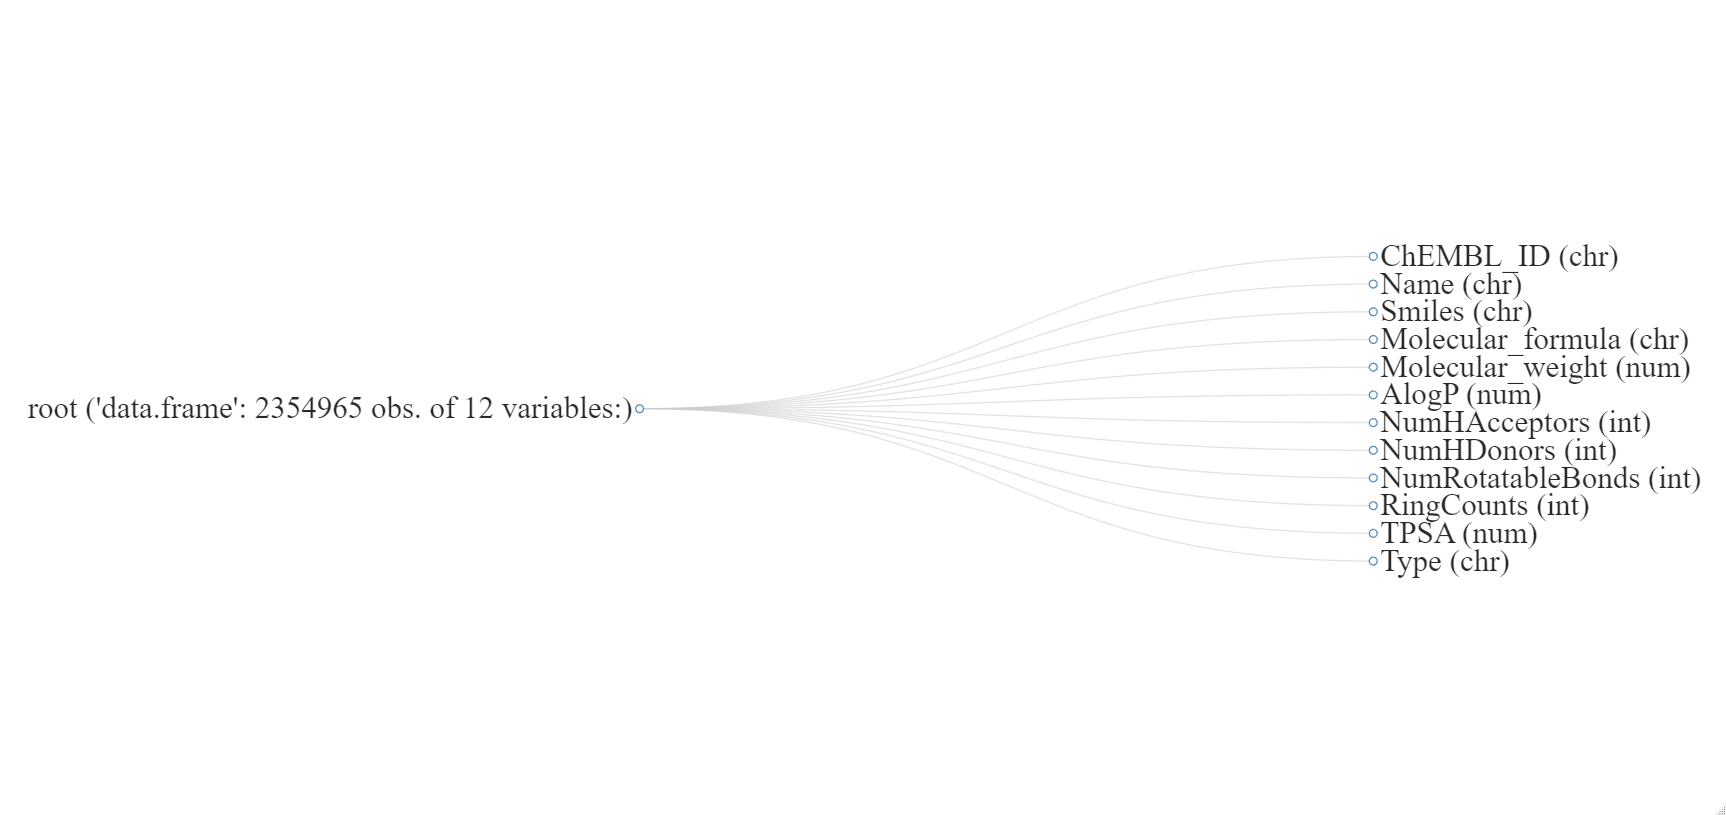
\includegraphics[width=0.8\textwidth]{variables.png}
  \caption{Studied Variables.}
\end{figure}

\section{Histograms of the quantitative variables}
\subsection{Histograms}
\begin{figure}[h]
  \centering
  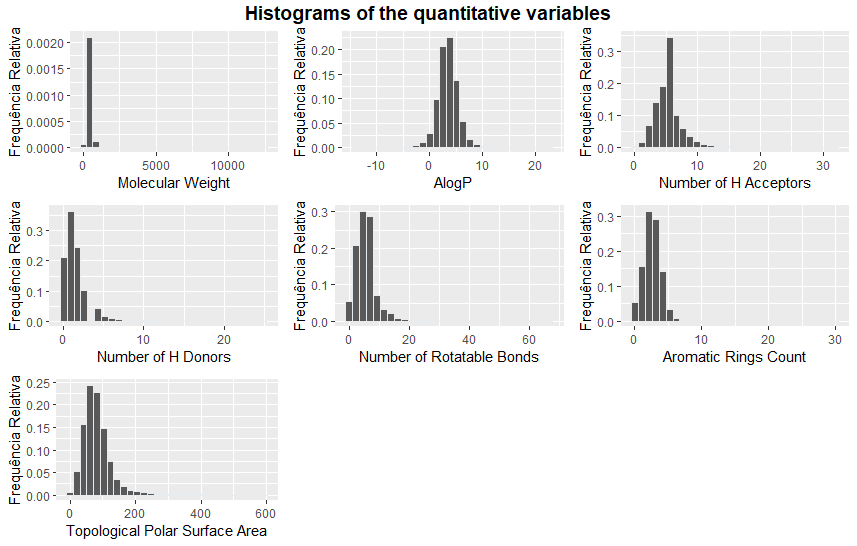
\includegraphics[width=\textwidth, height = 270pt]{histogram.png}
  \caption{Histograms}
\end{figure}
\newpage
\subsection{Trimmed Histograms}
\begin{figure}[h]
  \centering
  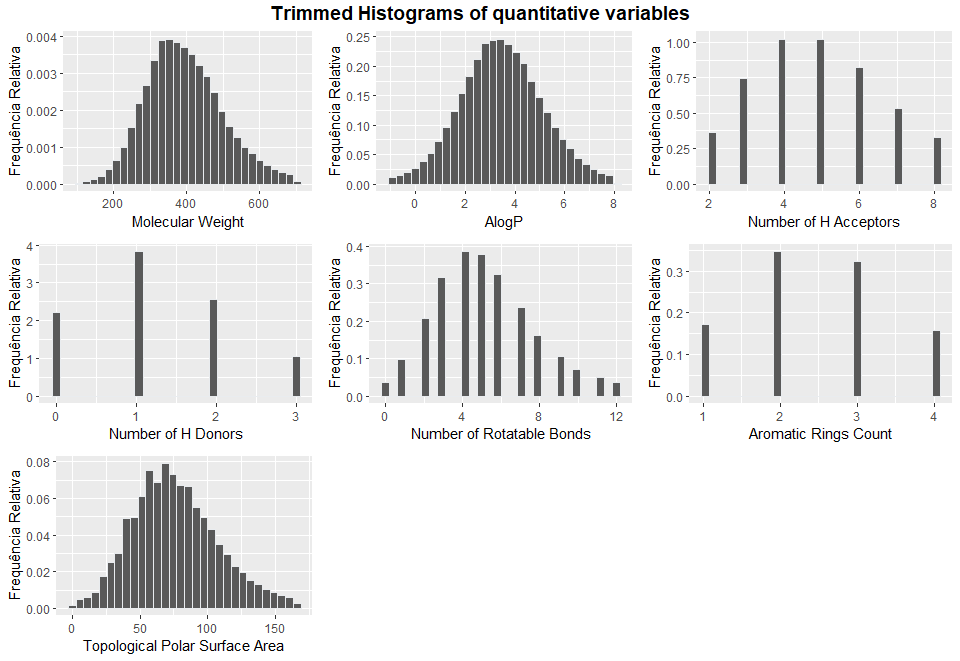
\includegraphics[width=\textwidth, height = 200pt]{trimmed.png}
  \caption{Trimmed Histograms}
\end{figure}

\section{Boxplot of the quantitative variables grouped by type of molecule}
\begin{figure}[h]
  \centering
  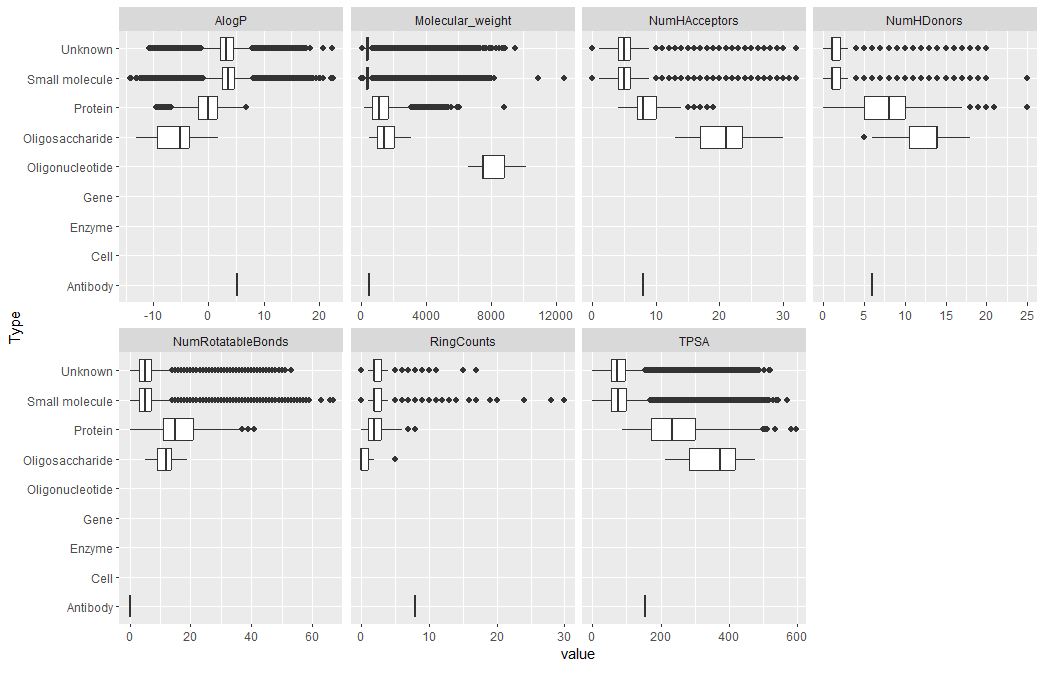
\includegraphics[width=\textwidth, height = 230pt]{boxplot.png}
  \caption{Boxplot}
\end{figure}

\newpage

\section{Correlation Matrix of the quantitative variables}
\begin{figure}[h]
  \centering
  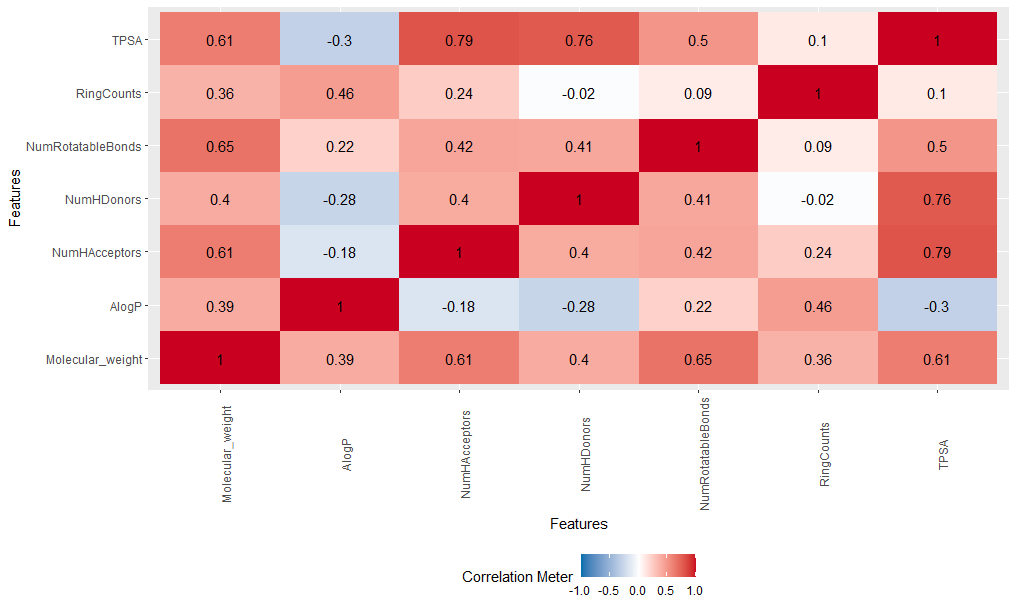
\includegraphics[width=\textwidth, height = 200pt]{correlation.png}
  \caption{Correlation Matrix}
\end{figure}

\section{Scatter plots with regression line}
\begin{figure}[h]
  \centering
  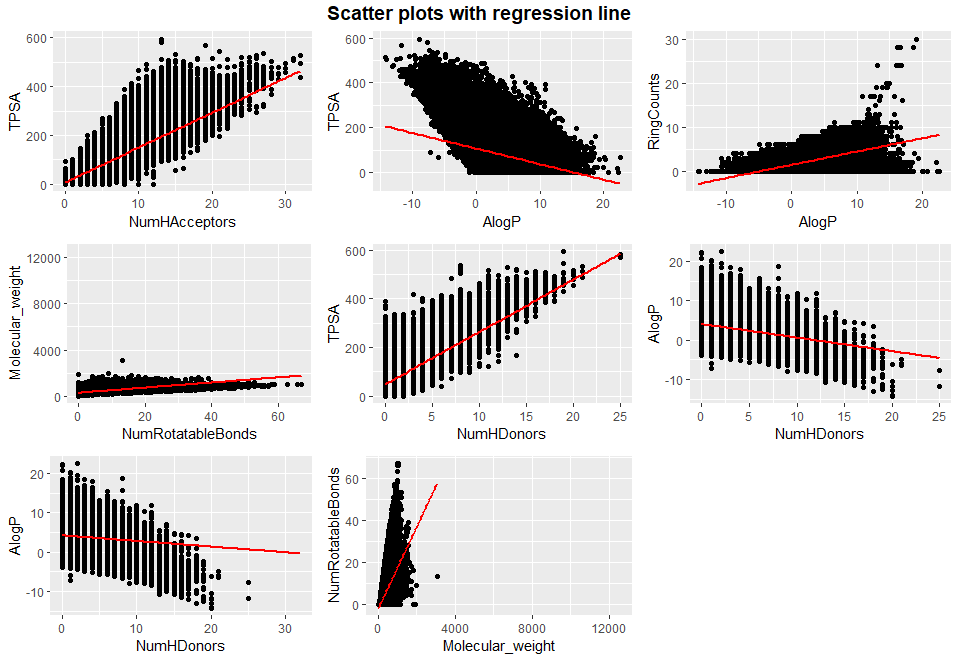
\includegraphics[width=\textwidth, height = 240pt]{regression.png}
  \caption{Correlation Matrix}
\end{figure}
\end{document}